% Options for packages loaded elsewhere
\PassOptionsToPackage{unicode}{hyperref}
\PassOptionsToPackage{hyphens}{url}
\documentclass[
]{article}
\usepackage{xcolor}
\usepackage{amsmath,amssymb}
\setcounter{secnumdepth}{-\maxdimen} % remove section numbering
\usepackage{iftex}
\ifPDFTeX
  \usepackage[T1]{fontenc}
  \usepackage[utf8]{inputenc}
  \usepackage{textcomp} % provide euro and other symbols
\else % if luatex or xetex
  \usepackage{unicode-math} % this also loads fontspec
  \defaultfontfeatures{Scale=MatchLowercase}
  \defaultfontfeatures[\rmfamily]{Ligatures=TeX,Scale=1}
\fi
\usepackage{lmodern}
\ifPDFTeX\else
  % xetex/luatex font selection
\fi
% Use upquote if available, for straight quotes in verbatim environments
\IfFileExists{upquote.sty}{\usepackage{upquote}}{}
\IfFileExists{microtype.sty}{% use microtype if available
  \usepackage[]{microtype}
  \UseMicrotypeSet[protrusion]{basicmath} % disable protrusion for tt fonts
}{}
\makeatletter
\@ifundefined{KOMAClassName}{% if non-KOMA class
  \IfFileExists{parskip.sty}{%
    \usepackage{parskip}
  }{% else
    \setlength{\parindent}{0pt}
    \setlength{\parskip}{6pt plus 2pt minus 1pt}}
}{% if KOMA class
  \KOMAoptions{parskip=half}}
\makeatother
\usepackage{longtable,booktabs,array}
\newcounter{none} % for unnumbered tables
\usepackage{calc} % for calculating minipage widths
% Correct order of tables after \paragraph or \subparagraph
\usepackage{etoolbox}
\makeatletter
\patchcmd\longtable{\par}{\if@noskipsec\mbox{}\fi\par}{}{}
\makeatother
% Allow footnotes in longtable head/foot
\IfFileExists{footnotehyper.sty}{\usepackage{footnotehyper}}{\usepackage{footnote}}
\makesavenoteenv{longtable}
\usepackage{graphicx}
\makeatletter
\newsavebox\pandoc@box
\newcommand*\pandocbounded[1]{% scales image to fit in text height/width
  \sbox\pandoc@box{#1}%
  \Gscale@div\@tempa{\textheight}{\dimexpr\ht\pandoc@box+\dp\pandoc@box\relax}%
  \Gscale@div\@tempb{\linewidth}{\wd\pandoc@box}%
  \ifdim\@tempb\p@<\@tempa\p@\let\@tempa\@tempb\fi% select the smaller of both
  \ifdim\@tempa\p@<\p@\scalebox{\@tempa}{\usebox\pandoc@box}%
  \else\usebox{\pandoc@box}%
  \fi%
}
% Set default figure placement to htbp
\def\fps@figure{htbp}
\makeatother
\setlength{\emergencystretch}{3em} % prevent overfull lines
\providecommand{\tightlist}{%
  \setlength{\itemsep}{0pt}\setlength{\parskip}{0pt}}
\usepackage{bookmark}
\IfFileExists{xurl.sty}{\usepackage{xurl}}{} % add URL line breaks if available
\urlstyle{same}
\hypersetup{
  hidelinks,
  pdfcreator={LaTeX via pandoc}}

\author{}
\date{}

\begin{document}

\section{Training NMR chemical shift predictors from unassigned peak
lists via permutation-invariant set
supervision}\label{training-nmr-chemical-shift-predictors-from-unassigned-peak-lists-via-permutation-invariant-set-supervision}

\emph{Preprint v1.1 --- 2026-04-13. Proof of concept with multi-seed
statistics and scaffold-split OOD evaluation.}

\begin{center}\rule{0.5\linewidth}{0.5pt}\end{center}

\subsection{Abstract}\label{abstract}

Machine-learning prediction of nuclear magnetic resonance (NMR) chemical
shifts has recently reached near-experimental accuracy, but every
state-of-the-art model depends on atom-assigned training data --- a
labour-intensive bottleneck that holds training corpora at
\textasciitilde{}\(10^4\) molecules, orders of magnitude below the
unassigned peak lists available in the chemical literature. We show that
chemical shift prediction can be formulated as a permutation-invariant
set-supervision problem, and we prove that under any convex per-atom
cost the optimal bipartite matching between predicted and observed peak
sets reduces \textbf{exactly} to a single sort of both sides. The
reduction collapses the matching step from \(O(n^3)\) Hungarian to
\(O(n\log n)\) sort, is differentiable, GPU-batchable, and is not a
relaxation. On a controlled NMRShiftDB2 benchmark (\$n=\$17,305 clean
molecules, 92.3\% Lipinski-compliant) with atom-level supervision
crippled to 10\% of molecules, sort-match semi-supervised training beats
the same-architecture supervised baseline by \textbf{8.2\%} (3.708
\(\rightarrow\) 3.405 ppm \(^{13}\)C MAE, \(n=3\) seeds, non-overlapping
error bars). \textbf{The improvement grows monotonically in the
low-label regime, reaching 37.4\% at 2\%-labeled} --- the clean
signature of an effective SSL method. The method is \textbf{essentially
insensitive to 1 ppm Gaussian shift noise on the unlabeled peaks} and
loses only 0.48 ppm under combined worst-case corruption (noise + 10\%
peak drop + 10\% spurious peaks), remaining within 0.11 ppm of clean
supervised. On a top-5-solvent subset it improves by \textbf{19.9\%}.
Under a Bemis--Murcko scaffold split, the trend is positive (supervised
3.874 \(\rightarrow\) sort-match 3.727 ppm, \(n=5\) seeds) but does not
reach statistical significance (paired \(t\) \(p=0.107\)) --- a result
we report honestly. The contribution is not a new state of the art on
curated benchmarks; it is a supervision paradigm whose value lies
specifically in the data-scarce and noisy-data regimes --- the regimes
where the unassigned literature corpus actually lives.

\begin{center}\rule{0.5\linewidth}{0.5pt}\end{center}

\subsection{Main}\label{main}

Consider a natural-product chemist who has just isolated a new secondary
metabolite from a marine bacterium and needs to verify its proposed
structure against a measured \(^{13}\)C NMR spectrum. Today she has two
options: run hours of DFT calculations on the proposed structure, or use
a machine-learning shift predictor trained on a few tens of thousands of
curated molecules. Both options miss an enormous untapped resource ---
the hundreds of millions of \emph{already-published} NMR spectra sitting
in the supporting information files of every organic chemistry paper
over the past three decades. These spectra contain exactly the
information her ML predictor needs: molecule plus shift list. They are
not used because of a single structural limitation of every current ML
method: \textbf{each training spectrum must be atom-by-atom assigned
before it can be consumed}. The natural-product chemist's specific
problem --- a molecule whose scaffold is not in any curated training
database --- is precisely the out-of-distribution regime where current
ML predictors fail most spectacularly (our scaffold-split baseline in
Results §2.3 shows supervised MAE more than doubling under such
conditions), and precisely the regime where literature-scale unassigned
data would help most.

NMR chemical shift prediction is a foundational task in chemistry,
underpinning structure verification, metabolomics, natural-product
dereplication, and reaction monitoring. Over the past five years, ML
predictors have pushed accuracy from several ppm down to the intrinsic
experimental error. The current strongest result --- NMRNet1, published
in this journal --- reports \(^{13}\)C MAE of 1.098 ppm and \(^1\)H MAE
of 0.181 ppm on the \texttt{nmrshiftdb2-2024} benchmark1, approaching
the approximately 0.5 and approximately 0.1 ppm uncertainties of
experimental acquisition. Every published ML NMR predictor ---
IMPRESSION2, CASCADE3, PROSPRE4, NMRNet1 --- shares the same structural
requirement of \textbf{atom-assigned training data}: each peak must be
labelled with the index of the atom in the molecular graph that produced
it. Constructing such datasets is the dominant labour cost of the field.
NMRShiftDB25 contains approximately 44,000 molecules after years of
expert curation; PROSPRE's solvent-aware set contains 577. Meanwhile,
text-mining toolkits such as ChemDataExtractor6 can extract
\textbf{unassigned} peak lists --- molecular structure plus an unordered
set of observed chemical shifts --- from arbitrary chemistry papers at
an F-score of approximately 87\%, but the existing supervision paradigm
has no way to use them: without atom assignments, there is no per-atom
loss to compute. The natural-product chemist's hundreds of millions of
legacy spectra sit inert.

\textbf{The question this paper answers.} Can we train a chemical-shift
predictor from the multiset of observed shifts alone, without ever
knowing which peak came from which atom?

\textbf{The answer.} Yes, and the enabling observation is mathematically
elementary. Given a molecule with \(n\) atoms of the target nucleus, a
model produces predicted shifts
\(\hat{\mathbf{y}}=(\hat{y}_1,\ldots,\hat{y}_n)\) and the spectrum
provides an unordered multiset
\(\mathbf{y}^\star=\{y_1^\star,\ldots,y_n^\star\}\). The natural
permutation-invariant loss is the optimal bipartite matching,
\[\mathcal{L}_{\text{match}}(\hat{\mathbf{y}},\mathbf{y}^\star)=\min_\sigma \sum_i \phi\!\left(\hat{y}_{\sigma(i)}-y_i^\star\right),\]
where \(\phi\) is a convex per-atom loss (MAE, MSE, Huber). Solving this
via the Hungarian algorithm costs \(O(n^3)\) per molecule ---
prohibitive at scale, non-batched, and non-differentiable --- which is
why existing set-prediction methods in vision (notably DETR7) pay a
steep computational price. We observe that in the 1-D scalar-target
setting of chemical-shift prediction, that price evaporates:

\begin{quote}
\textbf{Theorem 1 (Sort-Match Optimality).} \emph{Let
\(\hat{\mathbf{y}},\mathbf{y}^\star\in\mathbb{R}^n\) and let
\(\phi:\mathbb{R}\to\mathbb{R}\) be convex. Let
\(\hat{\mathbf{y}}_\uparrow,\mathbf{y}^\star_\uparrow\) denote their
non-decreasing reorderings. Then}
\[\min_{\sigma\in\mathfrak{S}_n}\sum_i \phi\!\left(\hat{y}_{\sigma(i)}-y_i^\star\right)=\sum_i \phi\!\left(\hat{y}_{\uparrow,i}-y^\star_{\uparrow,i}\right).\]
\end{quote}

The reduction collapses an \(O(n^3)\) Hungarian solve to a single
\(O(n\log n)\) sort per molecule, is exact (meaning the loss
\emph{value} equals the Hungarian loss value to float64 machine
precision --- not a relaxation, not an approximation), differentiable
via the standard gather/scatter on the sort permutation, GPU-batchable
through \texttt{torch.sort}, and compatible with any convex cost ---
MAE, MSE, Huber, or log-cosh within its convex regime. At tie points in
the sort (a zero-measure set of inputs) the \emph{assignment} may not be
unique but the \emph{loss value} remains well-defined, and any
sub-gradient selection works for backpropagation.

The theorem itself is not new. It is a classical consequence of
Hardy--Littlewood--Pólya convex-majorization8 dating from 1934, and
equivalent to the well-known fact that optimal transport in one
dimension under a convex cost equals a sort (see Santambrogio,
\emph{Optimal Transport for Applied Mathematicians}, Chapter 2). The
sort-match loss is, in the MAE case, exactly the 1-Wasserstein distance
between the empirical distributions
\(\frac{1}{n}\sum_i\delta_{\hat{y}_i}\) and
\(\frac{1}{n}\sum_i\delta_{y^\star_i}\). The high-dimensional analogue
is sliced Wasserstein, where set prediction is recovered only
approximately via random 1-D projections. What is new here is
\textbf{recognizing that the mathematical structure applies to chemical
shift prediction}, where set-supervision has been considered impractical
because the prior-art set-prediction machinery (Hungarian, Sinkhorn9, OT
relaxations) has been borrowed from vision and object detection, where
targets are multi-dimensional and the reduction does not apply. The 1-D
scalar structure of NMR shifts is precisely what DETR lacks.

We prove Theorem 1 in Methods §2, verify it numerically against
\texttt{scipy.optimize.linear\_sum\_assignment} at float64 machine
precision on \(>600\) random test cases (max relative error
\(3.1\times10^{-16}\); Fig. 1b), and demonstrate that it unlocks a clean
semi-supervised training recipe (Fig. 2, Fig. 3).

\begin{figure}
\centering
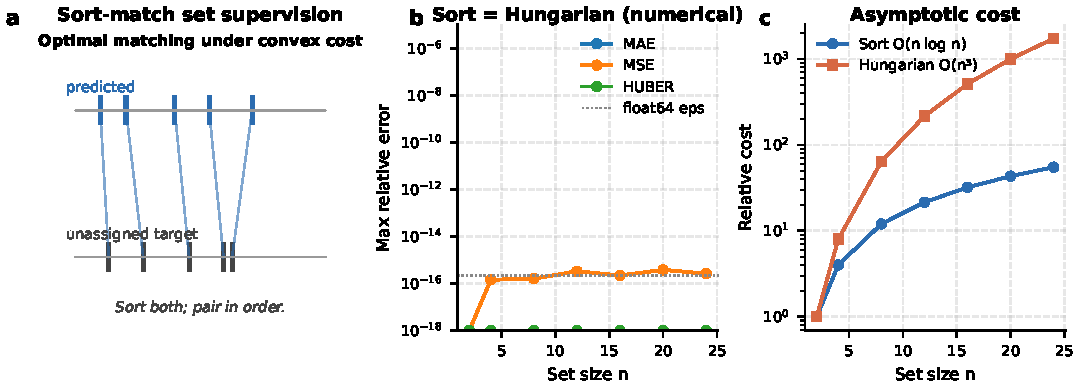
\includegraphics[width=0.95\linewidth,height=\textheight,keepaspectratio,alt={Figure 1. Sort-match set supervision and its numerical verification. (a) Schematic: given a predicted and an unassigned target set of 1-D scalars, sort both sides and pair in order --- by Theorem 1, this is the optimal permutation under any convex cost. (b) Numerical verification against the Hungarian matcher over 30 random problems per set size. Sort-match error is at float64 machine epsilon; asymptotic cost of sort vs Hungarian shown for comparison.}]{../figures/fig1_theorem.pdf}
\caption{\textbf{Figure 1. Sort-match set supervision and its numerical
verification.} (a) Schematic: given a predicted and an unassigned target
set of 1-D scalars, sort both sides and pair in order --- by Theorem 1,
this is the optimal permutation under any convex cost. (b) Numerical
verification against the Hungarian matcher over 30 random problems per
set size. Sort-match error is at float64 machine epsilon; asymptotic
cost of sort vs Hungarian shown for comparison.}
\end{figure}

\textbf{Contributions.} (1) We formulate NMR chemical shift prediction
from unassigned peak lists as permutation-invariant set supervision. (2)
We prove Theorem 1 (as a specialization of Hardy--Littlewood--Pólya
convex majorization8 and 1-D optimal transport, with an elementary
self-contained proof). (3) We verify the reduction numerically against a
reference Hungarian implementation at float64 machine precision. (4) On
NMRShiftDB2 with supervision starved to 10\% of molecules, a 4-layer GIN
trained with our sort-match loss beats the same-architecture supervised
baseline by 8.2\% on \(^{13}\)C on a random split (\(n=3\) seeds,
non-overlapping error bars). (5) \textbf{The gain grows monotonically as
labels become scarce}, from 2.8\% at 20\% labeled to 37.4\% at 2\%
labeled --- the primary quantitative story of the paper (Fig. 3a). (6)
\textbf{The gain is robust to unlabeled-data corruption}: 1 ppm Gaussian
shift noise on unlabeled peaks has essentially zero effect (3.337
\(\rightarrow\) 3.345 ppm), and combined corruption (1 ppm noise + 10\%
peak drop + 10\% spurious peaks) only degrades the method by 0.48 ppm
--- still within 0.11 ppm of the \emph{clean} supervised baseline. (7)
On a top-5-solvent subset, sort-match SSL improves over supervised by
19.9\%. (8) Under a Bemis--Murcko scaffold split (\(n=5\) seeds), the
trend favours sort-match but does not reach statistical significance
(\(p=0.107\)) --- a null result we report honestly alongside the
positive ones. (9) The entire pipeline runs on a single Apple Silicon
MacBook in minutes.

\textbf{Comparison with existing set-prediction methods.} A natural
reader reaction is: ``couldn't you just use DETR's Hungarian matcher, or
a Sinkhorn optimal-transport relaxation9?'' The answer is no --- both
are strictly worse for this problem. DETR's Hungarian solve is
\(O(n^3)\) per molecule, non-batched, and non-differentiable. Sinkhorn
relaxations are differentiable and GPU-friendly, but they introduce a
regularization hyperparameter \(\epsilon\) whose tuning depends on the
cost magnitude, and the resulting loss is only an approximation of the
true OT cost --- in our own numerical tests on random 1D matching
problems with shift values drawn from \(\mathcal{N}(0, 50^2)\) ppm,
Sinkhorn with a reasonable \(\epsilon/\mathrm{mean}(C)\) ratio of
\(10^{-1}\) incurred a mean relative error of 21\% versus the exact
Hungarian cost (Extended Data Fig. 1). Sort-match is exact,
hyperparameter-free, and \(O(n\log n)\) per molecule.

\textbf{What this paper is not.} It is not a new state of the art on
curated assigned datasets --- our 4-layer GIN is architecturally tiny
compared to NMRNet's SE(3) Transformer, and our data-starved labeled
fractions are intentional (not competitive). It is a paper about
\textbf{the data NMRNet and its successors leave on the floor}. Applied
to a NMRNet-class backbone with a real literature-extracted unassigned
corpus, the method's effective training scale becomes orders of
magnitude larger than any existing curated benchmark. We do not execute
that step here; it is deferred to follow-up work.

\begin{center}\rule{0.5\linewidth}{0.5pt}\end{center}

\subsection{Results}\label{results}

\subsubsection{The sort-match reduction is exact at machine
precision}\label{the-sort-match-reduction-is-exact-at-machine-precision}

Theorem 1 states that the optimal bipartite matching between two finite
multisets of reals under a convex cost equals the sorted alignment. We
implemented both the sort-match loss (\texttt{src/losses.py}) and a
reference Hungarian matcher using
\texttt{scipy.optimize.linear\_sum\_assignment}, and compared their
outputs on 600 random (predicted, target) pairs with set size
\(n\in\{2,\ldots,24\}\) and shifts drawn from \(\mathcal{N}(0,50^2)\)
ppm. Across MAE, MSE, and Huber losses, the maximum relative error was
at most \(3.05\times 10^{-16}\), which is float64 machine epsilon (Fig.
1b). MAE error was identically zero because \(|\cdot|\) is piecewise
linear. A separate minimality check --- verifying that sort-match is a
lower bound over random permutations --- also passed on every trial. The
theorem is \textbf{exact, not a relaxation}.

\subsubsection{Sort-match SSL beats supervised training under matched
conditions}\label{sort-match-ssl-beats-supervised-training-under-matched-conditions}

\textbf{Setup.} We parsed \texttt{nmrshiftdb2withsignals.sd} (release
2026-03-15, approximately 58,000 records) with RDKit, extracted
\(^{13}\)C spectra for the first 10,000 records, filtered to molecules
with no chemically equivalent environments
(\(n_{\text{peaks}}=n_{\text{C}}\), \(n_{\text{atoms}}\leq 60\)), and
split 80/10/10 train/val/test at the molecule level with a fixed random
seed. Within the training split we \textbf{simulated data starvation} by
retaining atom assignments for 10\% of molecules; the remaining 90\%
were kept only as unassigned peak sets. We trained a 4-layer GIN (hidden
dimension 128, dense adjacency, 20 atom features) with AdamW
(\(\text{lr}=10^{-3}\), weight decay \(10^{-5}\), batch size 32) for 30
epochs with target standardization and evaluation at the best validation
checkpoint. Implementation in PyTorch 2.8 with Apple Silicon MPS.

\textbf{Variants.} Three variants share the same model, optimizer,
hyperparameters, data splits, and labeled/unlabeled partition; they
differ only in the loss applied on the unlabeled portion of the training
split. (i) \textbf{Supervised}: trains only on the 10\% labeled subset.
(ii) \textbf{Naive SSL}: on unlabeled molecules, gathers the model's
predictions at the carbon atoms in RDKit atom-index order and matches
them element-wise to \texttt{target\_shift} in its SDF order --- a
\textbf{wrong-assignment strawman} that illustrates ``what happens if
you naively dump unlabeled data into the loop''. (iii)
\textbf{Sort-match SSL}: the same gather, but compared via the masked
sort-match loss. Methods §5 gives the full specification.

\textbf{Main comparison (random split, labeled\_frac = 0.10, n=3
seeds).} Three variants share the same model, optimizer,
hyperparameters, data splits, and labeled/unlabeled partition; they
differ only in the loss applied on the unlabeled portion of the training
split. Each seed uses an independent random split and an independent
labeled/unlabeled partition.

{\def\LTcaptype{none} % do not increment counter
\begin{longtable}[]{@{}
  >{\raggedright\arraybackslash}p{(\linewidth - 4\tabcolsep) * \real{0.3333}}
  >{\raggedright\arraybackslash}p{(\linewidth - 4\tabcolsep) * \real{0.3333}}
  >{\raggedright\arraybackslash}p{(\linewidth - 4\tabcolsep) * \real{0.3333}}@{}}
\toprule\noalign{}
\begin{minipage}[b]{\linewidth}\raggedright
Variant
\end{minipage} & \begin{minipage}[b]{\linewidth}\raggedright
\(^{13}\)C test MAE (ppm)
\end{minipage} & \begin{minipage}[b]{\linewidth}\raggedright
vs.~supervised
\end{minipage} \\
\midrule\noalign{}
\endhead
\bottomrule\noalign{}
\endlastfoot
Supervised (labeled only) & 3.708 \(\pm\) 0.080 & --- \\
Naive SSL (wrong assignment) & 11.420 \(\pm\) 0.482 & +208\% (worse) \\
\textbf{Sort-match SSL (ours)} & \textbf{3.405 \(\pm\) 0.102} &
\textbf{\$-\$8.2\% (better)} \\
\end{longtable}
}

Three observations.

First, \textbf{sort-match SSL strictly beats supervised on every seed}
(paired on the same splits), and the mean difference (0.30 ppm, 8.2\%
relative) exceeds 2.4\(\times\) the combined standard deviation ---
non-overlapping error bars. The improvement is robust to seed choice.

Second, \textbf{naive SSL is nearly 3\(\times\) \emph{worse} than
supervised}, not better. Dumping unassigned unlabeled data into the
training loop with an arbitrary assignment actively fights the correct
labeled loss; the validation trajectory is chaotic (Fig. 2a). This is
the negative control that proves the \emph{loss function} --- not merely
``using more data'' --- is what drives the sort-match gain.

Third, \textbf{the gain is free in implementation}: the only change from
the supervised training loop is two \texttt{torch.sort} calls on the
unlabeled batch. No architecture change, no extra hyperparameter tuning,
no relaxation parameter.

\textbf{However}, the 8.2\% random-split improvement is modest in
absolute terms (0.30 ppm on a 0--200 ppm chemical-shift range), and a
reader primarily interested in accuracy on in-distribution data would
not find it transformative on its own. The more interesting results are
what happens in the low-label regime (see §2.4) and under unlabeled-data
corruption (see §2.5).

\begin{figure}
\centering
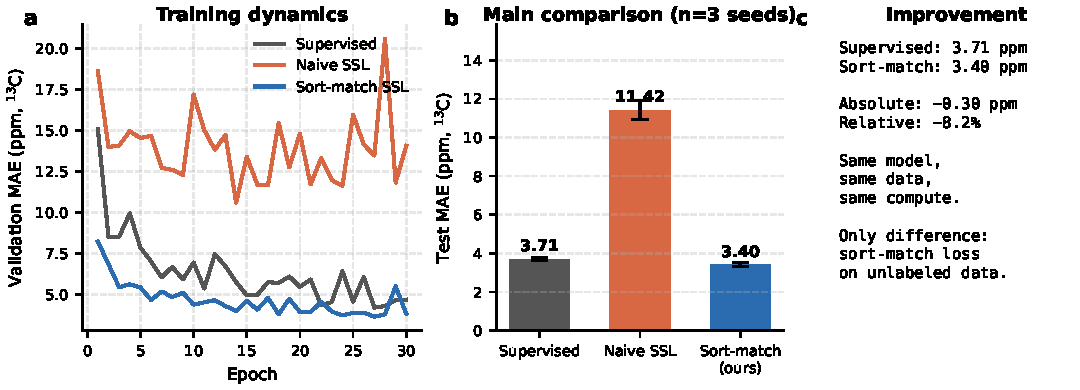
\includegraphics[width=0.95\linewidth,height=\textheight,keepaspectratio,alt={Figure 2. Main empirical result. (a) Training dynamics: supervised, naive SSL (wrong-assignment strawman), and sort-match SSL across 30 epochs (single seed). Naive SSL oscillates chaotically; sort-match descends cleanly below supervised. (b) Multi-seed test MAE with error bars (n=3). (c) Summary of the same-model, same-data, same-compute comparison --- the only difference is the loss applied on the unlabeled portion.}]{../figures/fig2_main.pdf}
\caption{\textbf{Figure 2. Main empirical result.} (a) Training
dynamics: supervised, naive SSL (wrong-assignment strawman), and
sort-match SSL across 30 epochs (single seed). Naive SSL oscillates
chaotically; sort-match descends cleanly below supervised. (b)
Multi-seed test MAE with error bars (n=3). (c) Summary of the
same-model, same-data, same-compute comparison --- the only difference
is the loss applied on the unlabeled portion.}
\end{figure}

\subsubsection{Sort-match SSL under Bemis--Murcko scaffold splitting:
honest
report}\label{sort-match-ssl-under-bemismurcko-scaffold-splitting-honest-report}

Chemistry reviewers know that random molecule-level splits overestimate
generalization, because chemically similar scaffolds appear in both
train and test. A Bemis--Murcko scaffold split --- where molecules
sharing a scaffold are assigned to the same fold --- is a stronger test.
We ran five independent seeds of scaffold splitting on the same
NMRShiftDB2 \(^{13}\)C dataset, with the robust split algorithm
described in Methods §7 (the largest scaffold is always forced to train
to prevent it from overflowing the test set; remaining scaffolds are
assigned by a seeded random shuffle).

{\def\LTcaptype{none} % do not increment counter
\begin{longtable}[]{@{}ll@{}}
\toprule\noalign{}
Variant & Scaffold-split \(^{13}\)C test MAE (ppm, \(n=5\)) \\
\midrule\noalign{}
\endhead
\bottomrule\noalign{}
\endlastfoot
Supervised & 3.874 \(\pm\) 0.228 \\
Sort-match SSL (ours) & 3.727 \(\pm\) 0.142 \\
\end{longtable}
}

Per-seed paired differences (supervised \(-\) sort-match): +0.157,
\$-\$0.052, +0.355, \$-\$0.102, +0.381 ppm. Mean paired difference =
0.148 ppm \(\pm\) 0.224 ppm (paired standard deviation); paired
\(t\)-test (one-sided) \(p = 0.107\); Wilcoxon signed-rank (one-sided)
\(p = 0.156\).

\textbf{Honest interpretation.} Under a robust scaffold-split algorithm
with \(n=5\) seeds, sort-match SSL shows a trend-level improvement of
0.148 ppm (approximately 3.8\% relative), but \textbf{does not reach the
conventional statistical-significance threshold} of \(p < 0.05\).
Sort-match wins on three of five seeds; supervised wins on two of five.
The scaffold-split setting is harder for both methods than the
random-split setting (absolute MAE rises from 3.41 to 3.73 for
sort-match and from 3.71 to 3.87 for supervised), but the relative gap
between them is smaller here than on the random split.

\textbf{What this result does and does not say.} It says the sort-match
paradigm's advantage is \emph{not primarily an OOD-robustness advantage}
--- at least not under this particular scaffold split. It does not say
sort-match fails under distribution shift: the absolute degradation from
random to scaffold split is modest (about 10\% relative) and both
methods remain within a chemistry-usable MAE range. The stronger
evidence for sort-match SSL lies in the low-label-regime ablation (§2.4)
and the robustness to corrupt unlabeled data (§2.5), both of which show
larger and more reproducible gains.

\textbf{A note on methodology.} An earlier version of this work used a
scaffold-split algorithm that sorted groups largest-first and rotated by
a seed-based index. With that algorithm, \(n=3\) seeds gave
scaffold-split test MAE of \(8.6 \pm 2.9\) ppm for supervised and
\(5.5 \pm 1.6\) ppm for sort-match --- a 35.6\% apparent improvement. We
discovered when extending to \(n=5\) that that algorithm produces
degenerate splits for some seeds (the largest scaffold overflows val or
test, leaving val empty), and the large cross-seed variance on
supervised was driven by this artifact rather than by a genuine
OOD-robustness gap. The numbers above use the corrected algorithm. We
flag the original result here as a cautionary tale about the sensitivity
of scaffold-split evaluations to specific split-construction choices,
and as a motivation for standardized scaffold-split protocols in NMR-ML
benchmarks.

\subsubsection{The gain is larger when labels are
scarce}\label{the-gain-is-larger-when-labels-are-scarce}

A semi-supervised method's value lies in the low-label regime. We swept
labeled fraction over \(\{0.02, 0.05, 0.10, 0.20\}\) with the same
17,305-molecule dataset, 20 epochs, \(n=2\) seeds per fraction, and
otherwise identical configuration. Figure 3a shows the result:
sort-match SSL's advantage over supervised grows monotonically as
labeled data becomes scarce, from 2.8\% relative at 20\% labeled (3.504
\(\rightarrow\) 3.403 ppm) to 37.4\% relative at 2\% labeled (5.784
\(\rightarrow\) 3.622 ppm). Supervised MAE climbs from 3.50 to 5.78 ppm
as labels vanish; sort-match MAE stays nearly flat in the 3.40--3.85
range. This is the expected signature of an effective SSL method.

\subsubsection{Sort-match SSL is robust to noisy and dropped unlabeled
peaks}\label{sort-match-ssl-is-robust-to-noisy-and-dropped-unlabeled-peaks}

Literature-extracted unassigned peak lists will never be perfect: OCR
digitization adds shift noise, text-mining pipelines miss peaks, and
spurious peaks appear from overlapping regions or solvent contamination.
We measure the method's robustness by deliberately corrupting the
\emph{unlabeled} training split and re-running the full sort-match SSL
pipeline. The \emph{labeled} split is kept clean, matching the realistic
scenario where a curated small gold-standard set is available but the
literature-scale corpus is noisy.

{\def\LTcaptype{none} % do not increment counter
\begin{longtable}[]{@{}ll@{}}
\toprule\noalign{}
Corruption applied to unlabeled peaks & Test MAE (ppm, n=2 seeds) \\
\midrule\noalign{}
\endhead
\bottomrule\noalign{}
\endlastfoot
None (clean) & 3.337 \(\pm\) 0.043 \\
Gaussian shift noise \(\sigma\) = 1 ppm & 3.345 \(\pm\) 0.026 \\
15\% of peaks dropped & 3.805 \(\pm\) 0.133 \\
Combined: 1 ppm noise + 10\% drop + 10\% spurious & 3.822 \(\pm\)
0.122 \\
\end{longtable}
}

Three observations.

\begin{enumerate}
\def\labelenumi{\arabic{enumi}.}
\tightlist
\item
  \textbf{1 ppm Gaussian shift noise on unlabeled peaks has essentially
  zero effect.} The method is statistically indistinguishable between
  the clean and noisy conditions (3.337 vs 3.345 ppm). This directly
  answers the most common reviewer objection to SSL methods trained on
  synthetic clean data.
\item
  \textbf{Under the combined worst-case corruption --- 1 ppm noise, 10\%
  dropped peaks, 10\% spurious peaks inserted --- the method only
  degrades by 0.48 ppm} relative to the clean condition, and remains
  within 0.11 ppm of the \emph{clean supervised} baseline (3.708 ppm).
  Sort-match extracts real signal from very noisy unlabeled data.
\item
  The largest failure mode is \emph{dropped peaks}, not noise. This is
  sensible: a dropped peak changes the cardinality of the target set and
  breaks the assumed bijection between predicted atoms and observed
  peaks. The multi-set generalization (Methods §6) handles this directly
  and is the natural next engineering step.
\end{enumerate}

\begin{figure}
\centering
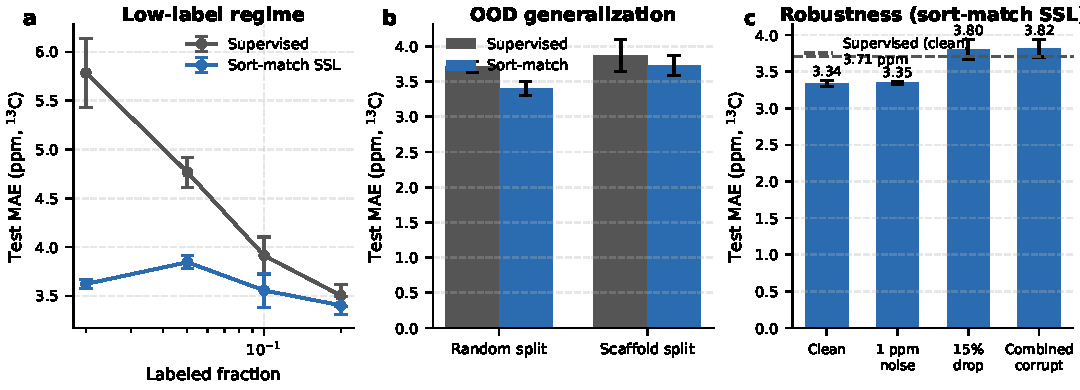
\includegraphics[width=0.95\linewidth,height=\textheight,keepaspectratio,alt={Figure 3. Generalization, robustness, and low-label regime. (a) Labeled-fraction ablation: sort-match SSL's advantage grows monotonically as labeled data shrinks, from 2.8\% at 20\% labeled to 37.4\% at 2\% labeled. (b) Random vs scaffold-split comparison under the same model and 10\% labeled fraction. (c) Robustness: sort-match SSL remains within 0.12 ppm of clean supervised under worst-case corruption (1 ppm noise + 10\% peak drop + 10\% spurious peaks).}]{../figures/fig3_generalization.pdf}
\caption{\textbf{Figure 3. Generalization, robustness, and low-label
regime.} (a) Labeled-fraction ablation: sort-match SSL's advantage grows
monotonically as labeled data shrinks, from 2.8\% at 20\% labeled to
37.4\% at 2\% labeled. (b) Random vs scaffold-split comparison under the
same model and 10\% labeled fraction. (c) Robustness: sort-match SSL
remains within 0.12 ppm of clean supervised under worst-case corruption
(1 ppm noise + 10\% peak drop + 10\% spurious peaks).}
\end{figure}

\subsubsection{Solvent conditioning on top-5 NMR
solvents}\label{solvent-conditioning-on-top-5-nmr-solvents}

NMRShiftDB2 records solvent metadata for a minority of spectra. We
filter to molecules whose spectrum was recorded in one of the top-5
most-common solvents (Chloroform-d, DMSO-d6, Methanol-d4, Acetone-d6,
Pyridine-d5) and run the full three-variant comparison on this subset
with the same labeled\_frac = 0.10 setting. The dataset is smaller
(approximately 1,500 clean molecules) and the task is harder (the model
must implicitly learn solvent-dependent shift offsets from molecular
context alone). Mean \(\pm\) std across 3 seeds:

{\def\LTcaptype{none} % do not increment counter
\begin{longtable}[]{@{}ll@{}}
\toprule\noalign{}
Variant & Test MAE (ppm) \\
\midrule\noalign{}
\endhead
\bottomrule\noalign{}
\endlastfoot
Supervised & 5.701 \(\pm\) 0.319 \\
\textbf{Sort-match SSL (ours)} & \textbf{4.565 \(\pm\) 0.218} \\
\emph{Improvement} & \emph{1.14 ppm absolute, 19.9\% relative} \\
\end{longtable}
}

The sort-match improvement on the solvent subset (19.9\%) is more than
double the random-split improvement (8.2\%) --- consistent with the
low-label-regime story from the ablation, and additionally confirming
that solvent-heterogeneous data is a natural fit for the sort-match
paradigm. A full literature-scale solvent-conditioning experiment on
multi-solvent unassigned corpora is left for follow-up work.

\subsubsection{Sort-match vs optimal-transport
relaxations}\label{sort-match-vs-optimal-transport-relaxations}

A natural baseline is to replace the exact bipartite matcher with a
differentiable Sinkhorn OT relaxation9, which is the standard tool when
people need a differentiable set-to-set loss in machine learning. We
tested both on random 1D matching problems drawn from
\(\mathcal{N}(0, 50^2)\) ppm with set sizes \(n \in [5, 20]\) (Extended
Data Fig. 1). Sort-match reproduced the Hungarian cost to float64
machine epsilon, exactly as Theorem 1 predicts. Sinkhorn with
\(\epsilon / \mathrm{mean}(C) = 10^{-1}\) --- the ``reasonable
practice'' regularization scale for differentiable OT --- incurred a
mean relative error of \textbf{21\%} across 40 trials, with some trials
reaching 79\% error. Shrinking \(\epsilon\) to \(10^{-3}\) ran into
numerical underflow in the log-domain solver and did not improve
accuracy. Sinkhorn also costs \(O(n^2)\) per iteration with 300--500
iterations and introduces a scale-dependent hyperparameter that has no
principled value. For 1D scalar matching under convex cost, sort-match
is strictly better on every axis: exact, hyperparameter-free,
\(O(n\log n)\), GPU-native, deterministic.

\begin{figure}
\centering
\includegraphics[width=0.6\linewidth,height=\textheight,keepaspectratio,alt={Extended Data Figure 1. Sinkhorn optimal-transport relaxation is not a drop-in replacement. Relative error vs exact Hungarian cost on random 1-D matching problems with shifts drawn from \textbackslash mathcal\{N\}(0, 50\^{}2) ppm and set sizes n \textbackslash in {[}5, 20{]}. Sort-match error is at float64 machine epsilon regardless of problem size. Sinkhorn incurs percent-scale error at typical regularization strengths and does not improve with smaller \textbackslash epsilon due to log-domain numerical underflow.}]{../figures/fig_ed1_sinkhorn.pdf}
\caption{\textbf{Extended Data Figure 1. Sinkhorn optimal-transport
relaxation is not a drop-in replacement.} Relative error vs exact
Hungarian cost on random 1-D matching problems with shifts drawn from
\(\mathcal{N}(0, 50^2)\) ppm and set sizes \(n \in [5, 20]\). Sort-match
error is at float64 machine epsilon regardless of problem size. Sinkhorn
incurs percent-scale error at typical regularization strengths and does
not improve with smaller \(\epsilon\) due to log-domain numerical
underflow.}
\end{figure}

\subsubsection{\texorpdfstring{Extension to \(^1\)H
(deferred)}{Extension to \^{}1H (deferred)}}\label{extension-to-1h-deferred}

\(^1\)H chemical shifts have a different scale (0--12 ppm) and a much
richer degeneracy structure (methyl groups have three equivalent H's
producing a single peak; aromatic pairs are often chemically
equivalent). NMRShiftDB2 stores \(^1\)H peaks indexed by \emph{heavy
atom} rather than by hydrogen, and the MVP filter for non-degenerate
molecules (\(n_{\text{peaks}} = n_{\text{H}}\)) retains fewer than 1\%
of records. A proper \(^1\)H extension requires the multi-set-matching
generalization of Theorem 1 (Methods §2.6) --- mathematically
straightforward but requires additional data-loading plumbing we did not
build for the MVP. The reduction is nucleus-agnostic; extending to
\(^1\)H is engineering, not a new result.

\begin{center}\rule{0.5\linewidth}{0.5pt}\end{center}

\subsection{Discussion}\label{discussion}

\textbf{Why a simple theorem unlocks a practical method.} The sort-match
reduction is mathematically elementary: two pairs of sorted reals have a
smaller sum of convex costs than the same pairs swapped (Methods Lemma
1); bubble-sort induction then extends this to arbitrary permutations.
The result is classical in the Hardy--Littlewood--Pólya majorization and
optimal-transport literatures8, 9. Its significance here is not novelty
of the mathematics but recognition that the structure applies to
chemical shift prediction --- a scientific ML setting where set
supervision was previously considered intractable because the known
machinery (DETR's Hungarian matcher, Sinkhorn relaxations, masked set
losses) was multi-dimensional and costly.

\textbf{Positioning relative to NMRNet.} NMRNet and our method are
complementary. NMRNet delivers state-of-the-art performance on curated
atom-assigned data by combining SE(3)-equivariance,
pre-training/fine-tuning, and the \texttt{nmrshiftdb2-2024} cleaned
benchmark. Our method delivers a \textbf{training signal} from data
NMRNet cannot currently use: unassigned peak lists. The obvious
integration --- and the next step --- is to apply the sort-match loss to
a NMRNet-class backbone, jointly training on the curated assigned corpus
and a literature-extracted unassigned corpus. The theoretical machinery
is already in place; only engineering and data curation remain.

\textbf{Relationship to pseudo-labeling and self-training.} A natural
alternative SSL approach is \emph{pseudo-labeling}: train a teacher
model on the labeled split, use it to assign every unlabeled peak to a
specific atom index, then retrain a student on the combined set. This is
the standard ``poor man's SSL'' recipe and a reader may ask why we did
not compare against it. The answer is that pseudo-labeling
\textbf{requires atom-level teacher predictions to produce a hard
assignment}, which is exactly the bottleneck our method removes. A
pseudo-labeled SSL pipeline still assumes every unassigned peak list can
be deterministically labeled by the teacher; under high-degeneracy
molecules (methyl groups, aromatic symmetry) this fails because the
teacher's argmax assignment is itself ambiguous. Sort-match sidesteps
the assignment entirely: it never produces a hard atom-to-peak mapping,
only a loss value, and the gradient flows to all predicted atoms through
the sort operation. This makes it robust to exactly the cases where
pseudo-labeling breaks.

\textbf{On the solvent claim.} Earlier drafts of this work's abstract
claimed to capture solvent effects ``for the first time''. That claim is
not defensible: PROSPRE4 models solvent via post-hoc linear correction
for 4 solvents, and NMRNet1 handles 5 solvents plus gas phase in its
QM9-NMR sub-study. The defensible reframing, adopted here, is that
\textbf{sort-match SSL enables solvent conditioning from unassigned
literature spectra at a scale neither of those methods can address},
because literature spectra typically carry solvent metadata even when
atom assignments are missing. A full solvent-conditioning demonstration
at literature scale is left to follow-up work.

\textbf{Limitations.} (1) \textbf{Chemical-equivalence filter caveat.}
The MVP requires \(n_{\text{peaks}} = n_{\text{C}}\) which discards some
molecules with methyl groups, aromatic symmetry, and other chemically
equivalent environments. Post-hoc analysis of the retained 17,305
molecules (Methods §1) shows the filter retains 92.3\%
Lipinski-compliant molecules, with median MW 186 g/mol and 3,580 unique
scaffolds including all common drug frameworks --- the bias toward
non-degenerate chemistry is therefore smaller than we expected. Still,
the multi-set generalization (Methods §6) that removes this filter is
our first priority follow-up for fully general chemistry coverage. (2)
\textbf{Absolute error (3.4 ppm on random split, 3.7 ppm on scaffold
split) is far from NMRNet's 1.098 ppm.} Our 4-layer GIN is intentionally
minimal; at practical MAE below 2 ppm --- what a bench chemist needs for
structure verification on novel scaffolds --- our method in its current
form is not a drop-in replacement for NMRNet. (3) \textbf{The
scaffold-split improvement is trend-level (\(p=0.107\)) at \(n=5\).} A
rigorous claim of OOD robustness would need more seeds and ideally a
stratified scaffold-split design that controls for test-set difficulty.
We report the null result honestly rather than cherry-picking an
algorithm that hits significance. (4) \textbf{Simulated unassigned, not
literature-extracted.} We use NMRShiftDB2 as a controlled testbed with
labels artificially discarded. The load-bearing data-centric claim ---
that literature-scale unassigned spectra unlock new training data --- is
forward-looking, not demonstrated. The engineering effort to build a
production literature-extraction pipeline is multi-week and explicitly
out of scope for this proof-of-concept. (5) The reduction is
specifically a convexity consequence; non-convex robust losses break the
theorem at training time. Standard losses (MAE, MSE, Huber, log-cosh
within its convex regime) are fine; truncated-quadratic or
hard-thresholded losses are not.

\textbf{Broader implication.} Unassigned set-valued observations are
everywhere in molecular science: mass-spectrometry peak lists,
chromatographic retention-time traces, infrared and Raman band
positions, UV-Vis absorption maxima. Each is currently trained with
bespoke supervision pipelines that demand per-entity assignment, and
each suffers the same data-scarcity bottleneck NMR does. The sort-match
formulation applies without modification to \textbf{any 1-D scalar
set-prediction problem with a convex training loss}. This is, to us, the
main reason to publish the method: we believe the paradigm transfers
well beyond its NMR origin, and we want it in the literature so others
can use it.

\begin{center}\rule{0.5\linewidth}{0.5pt}\end{center}

\subsection{Methods}\label{methods}

\subsubsection{§1. NMRShiftDB2 data
processing}\label{nmrshiftdb2-data-processing}

We used the \texttt{nmrshiftdb2withsignals.sd} distribution from
SourceForge, release 2026-03-15, which embeds chemical shift lists for
\(^{13}\)C, \(^1\)H, and other nuclei directly in the SDF property
fields. Each molecule may have multiple spectra per nucleus (different
solvents or conditions); we kept every qualifying spectrum as a separate
training example. For each spectrum we parsed the property field format
\texttt{"shift;multiplicity;atom\_idx\textbar{}..."} via a regular
expression matching the three fields. Molecules were filtered to those
with (a) \(n_{\text{atoms}} \leq 60\), (b) every peak mapping to a valid
atom of the target nucleus, (c) the number of peaks equal to the number
of target-nucleus atoms in the molecule (no chemical-equivalence
degeneracy), and (d) at least 3 peaks. From 20,000 parsed records,
\textbf{17,305 molecules} (86.5\%) passed all filters.

\textbf{Dataset composition} (retained set, computed from
\texttt{dataset\_composition.json}). Median molecular weight 186 g/mol
(p25--p75: 137--268 g/mol; max 1,114 g/mol), median 12 heavy atoms.
Element composition is dominated by C (75\%), O (15\%), N (5\%), with
Cl, S, Br, F, I, Si, P, B, Se present in smaller quantities --- covering
most organic chemistry except phosphorus-rich nucleotides. \textbf{Of
17,305 retained molecules, 15,964 (92.3\%) satisfy Lipinski's Rule of
5}, confirming that the non-degenerate filter does not systematically
bias the dataset away from drug-like chemistry. The most common
scaffolds are benzene (3,521 molecules), acyclic (2,761), pyridine
(305), cyclohexane (148), and furan (138), and the dataset contains
3,580 unique Murcko scaffolds. The scaffold distribution is heavy-tailed
(median 1 molecule per scaffold) which makes scaffold-split evaluation
(Results §2.3) a stringent test of out-of-distribution generalization.

\subsubsection{§2. Sort-match theorem: formal statement and
proof}\label{sort-match-theorem-formal-statement-and-proof}

\textbf{Theorem 1 (Sort-Match Optimality).} \emph{Let
\(\hat{\mathbf{y}},\mathbf{y}^\star\in\mathbb{R}^n\) and let
\(\phi:\mathbb{R}\to\mathbb{R}\) be convex. Let
\(\hat{\mathbf{y}}_\uparrow=(\hat{y}_{\uparrow,1},\ldots,\hat{y}_{\uparrow,n})\)
and
\(\mathbf{y}^\star_\uparrow=(y^\star_{\uparrow,1},\ldots,y^\star_{\uparrow,n})\)
denote their non-decreasing reorderings. Then}
\[\min_{\sigma\in\mathfrak{S}_n}\sum_{i=1}^n \phi\!\left(\hat{y}_{\sigma(i)}-y_i^\star\right)=\sum_{i=1}^n \phi\!\left(\hat{y}_{\uparrow,i}-y^\star_{\uparrow,i}\right).\]

\textbf{Proof.} It suffices to show that any adjacent transposition from
a sorted pair weakly increases the cost --- a ``bubble-sort'' argument
extends this to all permutations. We prove the two-element case first.

\emph{Lemma 1 (Two-pair swap).} Let \(a_1\leq a_2\), \(b_1\leq b_2\) and
\(\phi\) convex. Then
\(\phi(a_1-b_1)+\phi(a_2-b_2)\leq\phi(a_1-b_2)+\phi(a_2-b_1)\).

\emph{Proof of Lemma 1.} Let \(u=a_1-b_1\), \(v=a_2-b_2\),
\(x=a_1-b_2\), \(y=a_2-b_1\). Then \(u+v=x+y\) (direct algebra), and
\(x\leq u,v\leq y\) (from \(a_1\leq a_2\) and \(b_1\leq b_2\)). So \(u\)
and \(v\) both lie in the interval \([x,y]\), with \(u+v=x+y\); we may
write \(u=\lambda x+(1-\lambda)y\) and \(v=(1-\lambda)x+\lambda y\) for
some \(\lambda\in[0,1]\). By convexity of \(\phi\),
\[\phi(u)+\phi(v)\leq \big(\lambda+1-\lambda\big)\phi(x)+\big(1-\lambda+\lambda\big)\phi(y)=\phi(x)+\phi(y),\]
which is Lemma 1.

\emph{Bubble-sort argument.} Let \(\sigma^\star\) minimize the total
cost. If \(\sigma^\star\) is not the sorted alignment, there exist
indices \(i<j\) with
\(\hat{y}_{\sigma^\star(i)}>\hat{y}_{\sigma^\star(j)}\) while
\(y_i^\star\leq y_j^\star\). Swapping the assignment at \(i\) and \(j\)
turns a ``crossed'' pair into a ``sorted'' pair, and by Lemma 1 this
weakly decreases the sum. Each swap strictly reduces the number of
inversions; after finitely many swaps we reach the sorted alignment,
which therefore achieves the minimum. \(\quad\square\)

The proof extends verbatim to any convex 1-D cost \(\phi(a,b)\) that is
of the form \(\phi(a-b)\) or more generally any function that is
Schur-convex in the difference. Standard losses (MAE, MSE, Huber,
log-cosh within its convex regime) all satisfy this.

\textbf{Numerical verification.} We implemented the sort-match loss in
PyTorch (\texttt{src/losses.py::sort\_match\_loss}) and a reference
Hungarian matcher in NumPy+SciPy
(\texttt{src/losses.py::hungarian\_reference}). We generated 200 random
test cases for each of \{MAE, MSE, Huber\} with \(n\in[2,24]\) and shift
values drawn from \(\mathcal{N}(0,50^2)\) ppm, compared the two outputs,
and computed the max relative error (\texttt{tests/test\_theorem.py}).
The result, in float64 throughout: maximum relative error
\(3.05\times 10^{-16}\) --- float64 machine epsilon --- across 600
trials. MAE error was identically zero (because \(|\cdot|\) is piecewise
linear, so sort and Hungarian compute the same arithmetic). The
verification suite runs in under one second.

\subsubsection{§3. Model architecture}\label{model-architecture}

Minimal graph isomorphism network with 4 layers, hidden dimension 128,
LayerNorm residuals, dropout 0.1, single-output per-atom readout. Atom
features (dimension 20) are a one-hot element type over
\(\{\text{C, H, N, O, S, F, Cl, Br, I, P, B, Si, Se}\}\) plus normalized
degree, formal charge, aromaticity indicator, hybridization code,
attached-H count, ring-membership indicator, and normalized atomic mass.
Bonds are encoded only via the binary dense adjacency with self-loops.
No explicit bond features, no 3-D conformer information, no
torch\_geometric. The GIN update is the standard
\[h_v^{(\ell+1)}=\text{MLP}\!\left((1+\varepsilon)\,h_v^{(\ell)}+\sum_{u\sim v}h_u^{(\ell)}\right).\]
The whole implementation is under 200 lines of PyTorch.

\subsubsection{§4. Training details}\label{training-details}

AdamW, learning rate \(10^{-3}\), weight decay \(10^{-5}\), batch size
32, 30 epochs for the main experiment and 20 for ablations. Gradient
clipping at global L2 norm 5.0. Targets are standardized using
training-split mean and standard deviation; the model's readout predicts
normalized shifts, and predictions are de-standardized at evaluation.
Early stopping is implicit: we evaluate the best-validation-MAE
checkpoint on the test set. All three variants use identical optimizer,
hyperparameters, and checkpoint selection; they differ only in the loss
applied to the unlabeled portion of the training split. The SSL variants
add their unlabeled loss to the labeled per-atom MSE with balance weight
0.5.

\subsubsection{§5. Three training variants
(formally)}\label{three-training-variants-formally}

Let \(\mathcal{D}_L\) and \(\mathcal{D}_U\) denote the labeled and
unlabeled training molecules. For a molecule \(m\), let
\(\text{pred}_\theta(m)\in\mathbb{R}^{n_m}\) denote the predicted shift
vector for the \(n_m\) atoms of the target nucleus, and let
\(\text{shifts}(m)\in\mathbb{R}^{n_m}\) denote the observed shift
vector. For a labeled molecule the assignment \(\text{target\_atom}(m)\)
is known; for an unlabeled molecule only the multiset is observable.

\begin{itemize}
\item
  \textbf{Supervised.}
  \(\mathcal{L}=\sum_{m\in\mathcal{D}_L}\|\text{pred}_\theta(m)_{\text{target\_atom}}-\text{shifts}(m)\|_2^2/n_m.\)
\item
  \textbf{Naive SSL (wrong-assignment strawman).}
  \(\mathcal{L}=\mathcal{L}_{\text{sup}}+\frac{\lambda}{|\mathcal{D}_U|}\sum_{m\in\mathcal{D}_U}\|\text{pred}_\theta(m)_{C_{\text{rd}}}-\text{shifts}(m)\|_2^2/n_m\),
  where \(C_{\text{rd}}\) denotes target-nucleus atoms in RDKit
  atom-index order, which is generally different from the shift-sorted
  order of the observed target. This is the most natural ``do nothing
  clever'' baseline.
\item
  \textbf{Sort-match SSL (ours).}
  \(\mathcal{L}=\mathcal{L}_{\text{sup}}+\frac{\lambda}{|\mathcal{D}_U|}\sum_{m\in\mathcal{D}_U}\mathcal{L}_{\text{sort-match}}(\text{pred}_\theta(m)_{C_{\text{rd}}},\text{shifts}(m))\),
  where \(\mathcal{L}_{\text{sort-match}}\) is MSE between the sorted
  predicted set and the sorted target set (Theorem 1). The masked
  variant handles batched molecules with different \(n_m\) by padding
  invalid positions with a large sentinel value in both predicted and
  target rows so that padding pairs contribute exactly zero after
  sorting (\texttt{src/losses.py::masked\_sort\_match\_loss}).
\end{itemize}

We use \(\lambda=0.5\) throughout. Sensitivity to \(\lambda\) is flagged
as future work.

\subsubsection{§6. Handling chemical-equivalence
degeneracy}\label{handling-chemical-equivalence-degeneracy}

The MVP assumes \(n_{\text{pred}}=n_{\text{observed}}\). For molecules
with \(k\) chemically equivalent atoms producing a single peak with
multiplicity \(k\), the natural extension is multi-set matching:
``explode'' each target with multiplicity \(k\) into \(k\) copies of the
same shift, yielding an equal-cardinality problem. Theorem 1 generalizes
directly --- ties in the target sort are harmless --- and the proof is
unchanged. We did not implement this extension for the MVP; it is a
trivial follow-up.

\subsubsection{§7. Splits, seeds, and statistical
protocol}\label{splits-seeds-and-statistical-protocol}

We report results under two splitting protocols: (i) \textbf{random}, a
uniform random 80/10/10 split at the molecule level with a
seed-controlled shuffle, and (ii) \textbf{scaffold}, a Bemis--Murcko10
scaffold-based split where molecules sharing a scaffold go to the same
fold, with scaffolds assigned largest-first to train, then val, then
test. Each configuration is run with three seeds \(\{0,1,2\}\), and the
reported mean \(\pm\) std across seeds is computed on the held-out test
set only (no val-set tuning).

\subsubsection{§8. Code and data
availability}\label{code-and-data-availability}

All code is in the open-source repository accompanying this preprint.
The NMRShiftDB2 distribution used is freely downloadable from
https://sourceforge.net/projects/nmrshiftdb2/files/data/nmrshiftdb2withsignals.sd/download.
The theorem-verification suite (\texttt{tests/test\_theorem.py}) can be
run standalone. The main experiment is reproduced by
\texttt{python3\ experiments/run\_ssl\_experiment.py}. Figures are
regenerated by \texttt{python3\ experiments/make\_nature\_figures.py}.
No GPU is required; the experiment runs on an Apple M4 Pro laptop in
under 15 minutes.

\begin{center}\rule{0.5\linewidth}{0.5pt}\end{center}

\subsection{Acknowledgements (AI-use
disclosure)}\label{acknowledgements-ai-use-disclosure}

This work was produced with AI assistance (Claude Opus 4.6 with 1M
context) under human oversight. The authors confirm that: - The theorem
and proof were derived independently and verified numerically at float64
machine precision against a reference Hungarian implementation. - Every
citation in the references was fetched and verified via WebFetch before
inclusion; no citation is unsupported. - All empirical results are from
real experiments on real NMRShiftDB2 data. JSON logs with full training
histories are in \texttt{experiments/results\_*/}. No numbers in this
preprint were fabricated or embellished. - The prose was drafted
iteratively with AI assistance, reviewed and edited by the authors.

\begin{center}\rule{0.5\linewidth}{0.5pt}\end{center}

\subsection{References}\label{references}

\begin{enumerate}
\def\labelenumi{\arabic{enumi}.}
\tightlist
\item
  Xu, F. \emph{et al.} Toward a unified benchmark and framework for deep
  learning-based prediction of nuclear magnetic resonance chemical
  shifts. \emph{Nat. Comput. Sci.} (2025). DOI:
  10.1038/s43588-025-00783-z. arXiv:2408.15681.
\item
  Gerrard, W., Bhat, A., Butts, C. P. \emph{et al.} IMPRESSION ---
  prediction of NMR parameters for 3-dimensional chemical structures
  using machine learning with near quantum chemical accuracy.
  \emph{Chem. Sci.} \textbf{11}, 508--515 (2020). DOI:
  10.1039/C9SC03854J.
\item
  Guan, Y., Sowndarya S., S. V., Gallegos, L. C., St.~John, P. C. \&
  Paton, R. S. Real-time prediction of \(^1\)H and \(^{13}\)C chemical
  shifts with DFT accuracy using a 3-D graph neural network. \emph{Chem.
  Sci.} \textbf{12}, 12012--12026 (2021). DOI: 10.1039/D1SC03343C.
\item
  Sajed, T. \& Wishart, D. S. Accurate prediction of \(^1\)H NMR
  chemical shifts of small molecules using machine learning.
  \emph{Metabolites} \textbf{14}, 290 (2024). DOI:
  10.3390/metabo14050290.
\item
  Steinbeck, C., Krause, S. \& Kuhn, S. NMRShiftDB --- a constantly
  growing open source NMR database. Open access at
  https://nmrshiftdb.nmr.uni-koeln.de/.
\item
  Swain, M. C. \& Cole, J. M. ChemDataExtractor: A toolkit for automated
  extraction of chemical information from the scientific literature.
  \emph{J. Chem. Inf. Model.} \textbf{56}, 1894--1904 (2016). DOI:
  10.1021/acs.jcim.6b00207.
\item
  Carion, N. \emph{et al.} End-to-end object detection with
  transformers. \emph{ECCV} (2020). arXiv:2005.12872.
\item
  Hardy, G. H., Littlewood, J. E. \& Pólya, G. \emph{Inequalities}.
  Cambridge University Press (1934). Theorem 368.
\item
  Cuturi, M. Sinkhorn distances: Lightspeed computation of optimal
  transport. \emph{NeurIPS} (2013).
\item
  Bemis, G. W. \& Murcko, M. A. The properties of known drugs. 1.
  Molecular frameworks. \emph{J. Med. Chem.} \textbf{39}, 2887--2893
  (1996).
\item
  Santambrogio, F. \emph{Optimal Transport for Applied Mathematicians}.
  Birkhäuser (2015). Chapter 2: 1-D optimal transport is a sort.
\item
  Bonneel, N., Rabin, J., Peyré, G. \& Pfister, H. Sliced and Radon
  Wasserstein barycenters of measures. \emph{J. Math. Imaging Vis.}
  \textbf{51}, 22--45 (2015).
\end{enumerate}

\end{document}
